


\subsection{Our Parallel Dynamic Frontier Leiden}

Our prior study \cite{sahu2024dflouvain} presented a parallel implementation of the Dynamic Frontier (DF) approach, which, as above, utilized per-thread collision-free hash tables and capitalized on the weighted degrees of vertices and the total edge weights of communities as auxiliary information. In this work, we expand upon this, by applying it to Parallel Leiden\ignore{\cite{sahu2023gveleiden}} instead. The pseudocode for this is outlined in Algorithm \ref{alg:delta}, accompanied by an explanation provided in Section \ref{sec:our-delta}. Similar to our DS Leiden counterpart, it processes the (incrementally) marked vertices during the local-moving phase, but operates on all vertices during the refinement phase\ignore{(of the first pass)} of Leiden algorithm.

A straightforward approach of applying DF approach involves processing the affected vertices in the local-moving phase, refining communities in the next phase, until the local-moving phase appears to converge. For small batch updates, the local-moving phase may converge in a single pass, and thus, our algorithm would stop after the first pass. However, this results in the generated communities being cut-short after the refinement phase, and thus the returned communities have poor modularity. Note that, unlike DF Louvain, we should not stop after the local-moving phase --- the refinement phase must be run --- to avoid internally disconnected and badly connected communities. However, to obtain these, we must run the communities algorithm till the end. This allows us to obtain high quality and retain properties of the Leiden algorithm, We refer to this approach as \textit{Full Refine}.

However, if a batch update is small, it is likely that only a small number of communities are affected, and thus only a subset of communities need to be refined. In order to identify the subset of communities that need to be refined, we keep track of vertices which migrate from one community to another, during the local-moving phase, and mark both the source and target communities, of each migration, as changed. Such communities may have their sub-community structure changed. However, note that the community membership ID of each vertex, obtained from the local-moving phase may not necessarily be self-contained, i.e., community $c$ may not contain a vertex with ID $c$ --- vertex $c$ may have joined some other community. This can cause an issue for the refinement phase (in the refinement phase, we first need to make each vertex isolated, i.e., each vertex $i$ belongs to its own community $i$). This is because if we, say we reset the community vertex ID $c$ belongs to, but do not reset the community $c$, the vertex ID $c$ could continue to stay as an isolated community, while not being connected to the other vertices in community $c$. Worse still, it is possible two separate communities with the same ID $c$ are formed, while not being connected. It should be noted that this problem does to arise if we refine/reset all communities, but rather arises only if we refine a subset of communities.

To address this issue, we need to renumber each community $c$, such that vertex ID $c$ belongs to community $c$. One should be careful while renaming communities as such, since the community weights and the set of changed communities are marked based on the old communities --- so these need to be adjusted accordingly upon renumbering the communities.

We would now like to consider the impact of a batch update, upon the communities that need to be refined. Note that edge deletions within a community may trigger the community to split. However, if a community is isolated, the local-moving phase would not be able to identify a better community assignement for any of the vertices belonging to the community. Thus, the only way for such an isolated community to undergo a split is to refine such a community. But, since there are no community migrations, this community would not be marked for refinement, based on our discussion above. To address this, for edge deletions in the batch update belonging to the same community, we must mark the community as changed, in order for it to be refined after the local-moving phase. Further, if there are edge insertions to two separate regions of a community, it is likely that it may split to two separate communities. Such a community, therefore, must also be refined, i.e., for edge insertions in the batch update belonging to the same community, we should mark the community as changed. We refer to this approach as \textit{Sub Refine}.

However, the above approach does not improve the performance of DF Leiden, particularly for small batch updates. We note that, even for small batch updates, the aggregation phase of the algorithm consumes a significant portion of the runtime, bottlenecking the algorithm. This is mainly due to the fact selective refinement of communities results in a large disparity in the sizes of communities to be aggregated --- several communities are of small size, due to being refined, while a small number of communities remain significantly large --- since they were left out of the refinement phase, and must now be aggregated into a single super-vertex. Threads being assigned the work of aggregating such large communities into super-vertices have a significant workload. Thus it is important to ensure that such heavily loaded threads are assigned minimal other communities to process, in order to ensure good work balance. A straightforward way to achieve this is simply to use dynamic work scheduling, and assign work to threads (where each thread is being assigned a range of community IDs to aggregate) in smaller chunk sizes. However, using to small a chunk size could result in significant scheduling overhead. We experiment with chunk size of $2$ to $2048$, and observe a chunk size of $32$ to yield the best performance on average (for various batch sizes). We refer to this approach as \textit{Optimized}. Figure X shows the runtimes of the three approaches on varying batch sizes (for DF, DS, and ND Leiden).

NOTE: We apply the above procedure only to the first pass of Leiden algorithm, where the algorithm spends a significant portions of the runtime (how much). Figure X shows the runtime spent by the algorithm on different phases and passes of DF Leided for varying batch updates.


\subsection{Extending the Naive-dynamic (ND) approach to Parallel Leiden algorithm}

Our earlier work \cite{sahu2024dflouvain} presented a parallel version of the Naive-dynamic (ND) approach, which utilizes the weighted degrees of vertices and the total edge weights of communities as auxiliary information, as shown in Figure \ref{fig:about-auxiliary}. In this report, we extend it to Parallel Leiden algorithm \cite{sahu2023gveleiden}. The psuedocode for this is given in Algorithm \ref{alg:naive}, and its explanation in Section \ref{sec:our-naive}.

\begin{figure}[hbtp]
  \centering
  \subfigure{
    \label{fig:about-auxiliary--with}
    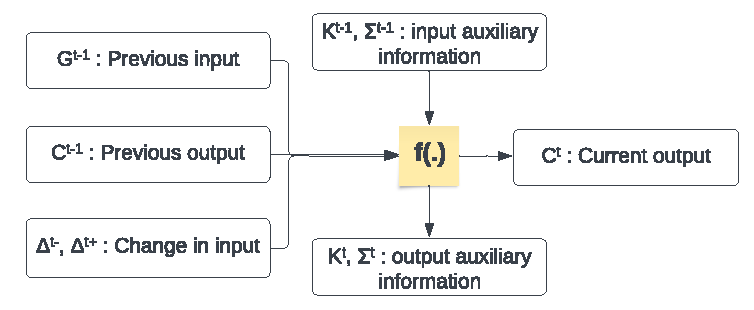
\includegraphics[width=0.98\linewidth]{out/about-auxiliary-with.pdf}
  } \\[-2ex]
  \caption{A dynamic community detection algorithm $f(.)$ takes as input the previous graph $G^{t-1}$, community memberships $C^{t-1}$, and the batch update $\Delta^{t-}$, $\Delta^{t+}$, and produces the updated community memberships $C^t$. However, it may also consider additional information such as the weighted degrees of vertices $K^{t-1}$ and the total edge weights of communities $\Sigma^{t-1}$ as auxiliary information, and yield updated auxiliary information $K^t$, $\Sigma^t$ \cite{sahu2024dflouvain}.}
  \label{fig:about-auxiliary}
\end{figure}





\subsection{Extending the Delta-screening (DS) approach to Parallel Leiden algorithm}

The Delta-screening (DS) approach proposed by Zarayeneh et al. \cite{com-zarayeneh21} is sequential. Our previous work \cite{sahu2024dflouvain} adapted it into an efficient parallel algorithm, which employed per-thread collision-free hash tables, and leveraged the weighted degrees of vertices and the total edge weights of communities as auxiliary information. Here, we extend this approach to Parallel Leiden algorithm \cite{sahu2023gveleiden}, by processing only the marked vertices during the local-moving phase, but processing all vertices during the refinement phase of the first pass\ignore{of the Leiden algorithm}. The psuedocode for this is in Algorithm \ref{alg:delta}, with a detailed explanation of the psuedocode given in Section \ref{sec:our-delta}.



\begin{figure}[!hbt]
  \centering
  \subfigure{
    \label{fig:optimize-subrefine--8020}
    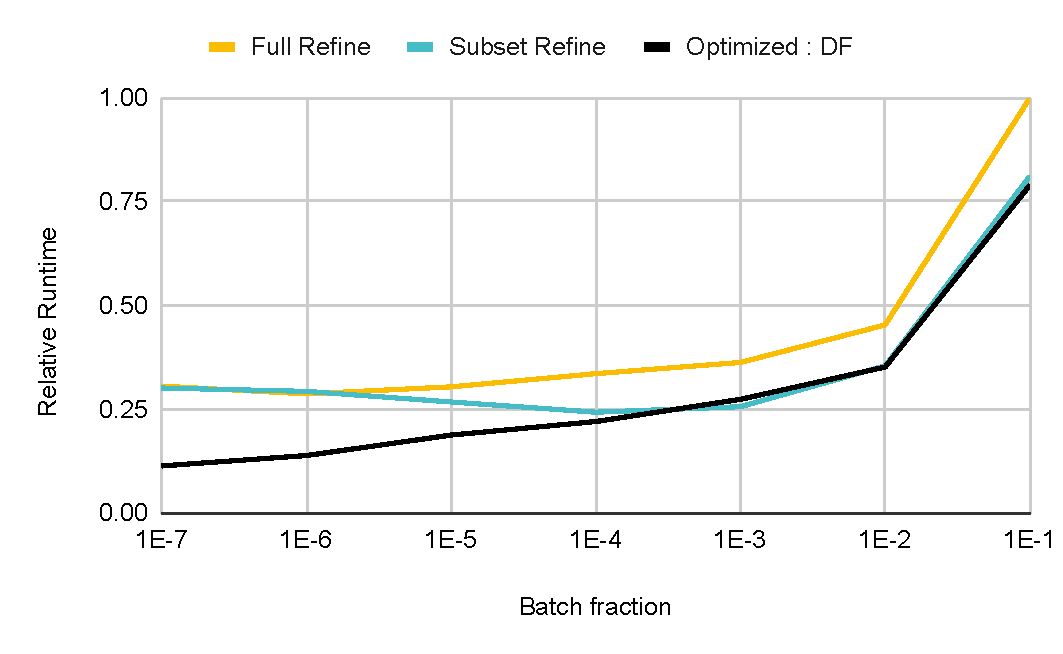
\includegraphics[width=0.98\linewidth]{out/optimize-subrefine-8020.pdf}
  } \\[-2ex]
  \caption{Mean Runtime and Modularity of communities obtained with our multicore implementation of \textit{Static}, \textit{Naive-dynamic (ND)}, \textit{Delta-screening (DS)}, and \textit{Dynamic Frontier (DF)} Leiden on real-world dynamic graphs, using batch updates of size $10^{-5}|E_T|$ to $10^{-3}|E_T|$. Here, (a) and (b) display the overall runtime and modularity across all temporal graphs, while (c) and (d) display the runtime and modularity for each individual graph. In (a), the speedup of each approach relative to Static Leiden is labeled.}
  \label{fig:optimize-subrefine}
\end{figure}

\begin{figure}[!hbt]
  \centering
  \subfigure[Relative runtimes on uniformly random batch updates of size $10^{-7}|E|$]{
    \label{fig:aggregation-adjust-chunksize--batch7}
    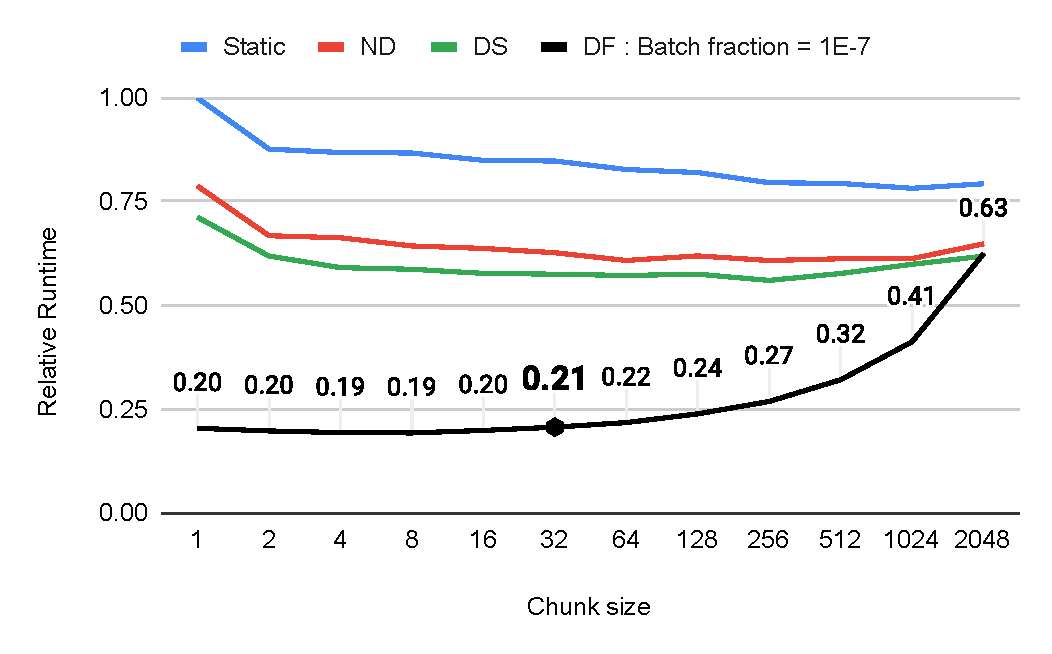
\includegraphics[width=0.98\linewidth]{out/aggregation-adjust-chunksize7.pdf}
  }
  \subfigure[Relative runtimes on uniformly random batch updates of size $10^{-5}|E|$]{
    \label{fig:aggregation-adjust-chunksize--batch5}
    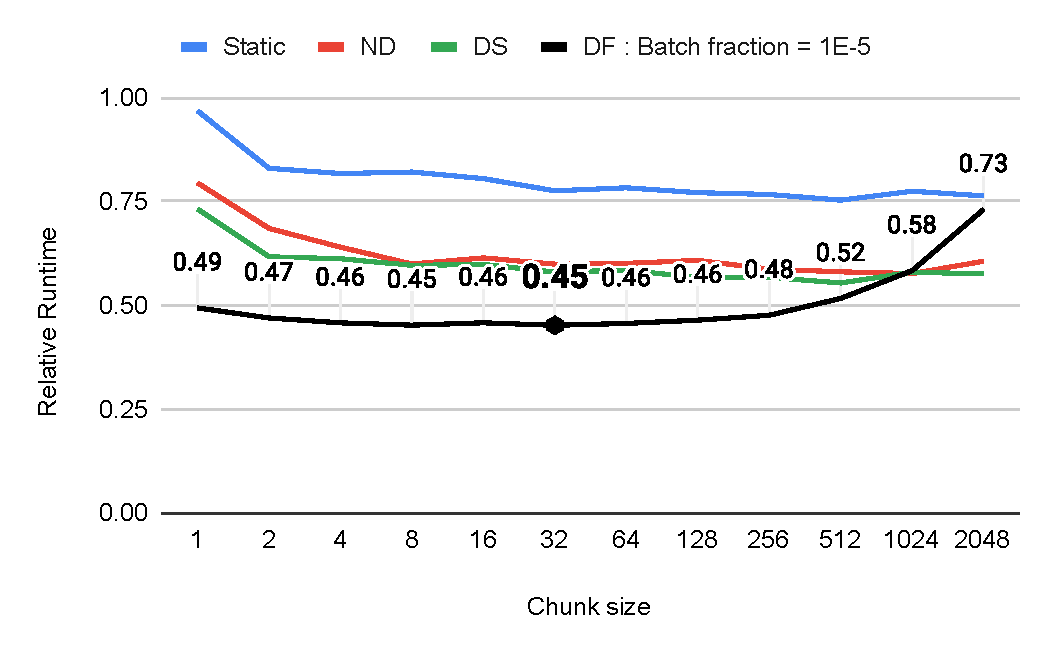
\includegraphics[width=0.98\linewidth]{out/aggregation-adjust-chunksize5.pdf}
  }
  \subfigure[Relative runtimes on uniformly random batch updates of size $10^{-3}|E|$]{
    \label{fig:aggregation-adjust-chunksize--batch3}
    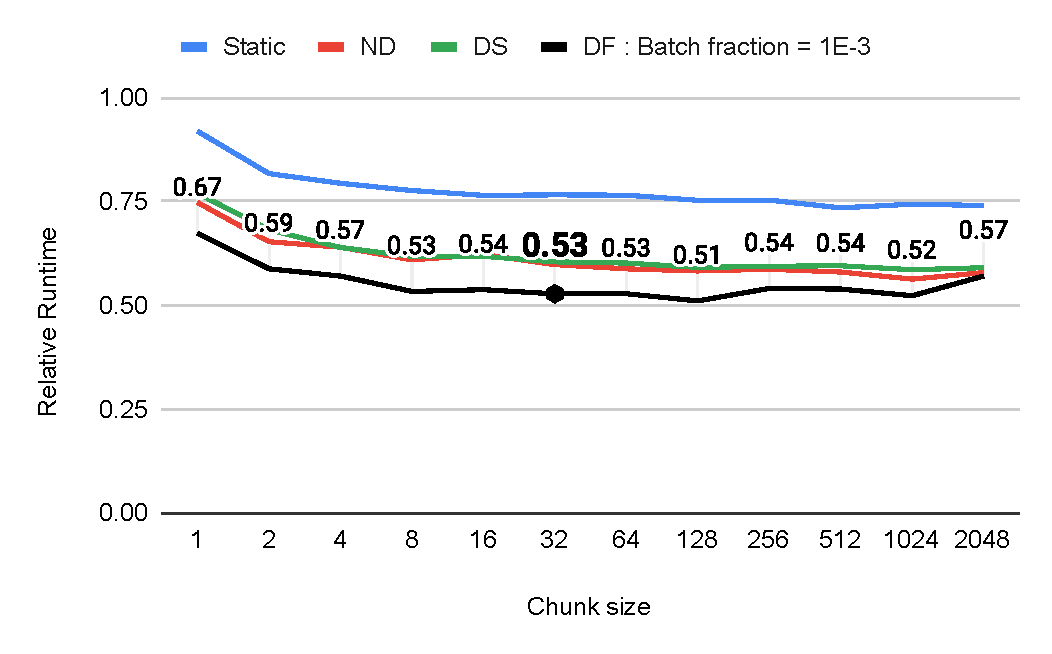
\includegraphics[width=0.98\linewidth]{out/aggregation-adjust-chunksize3.pdf}
  } \\[-1ex]
  \caption{Relative Runtime of \textit{Static}, \textit{Naive-dynamic (ND)}, \textit{Delta-screening (DS)}, and \textit{Dynamic Frontier (DF)} Leiden, with varying dynamic schedule chunk size (OpenMP), for aggregation phase of the Leiden algorithm. These tests were conducted on large graphs, with batch updates randomly generated at sizes of $10^{-7}|E|$, $10^{-5}|E|$, and $10^{-3}|E|$. The results suggest that a chunk size of $32$ is optimal (highlighted).}
  \label{fig:aggregation-adjust-chunksize}
\end{figure}

